% Seccion consolidada del TFM sobre sparsity 2:4. Incluir con % Seccion consolidada del TFM sobre sparsity 2:4. Incluir con % Seccion consolidada del TFM sobre sparsity 2:4. Incluir con % Seccion consolidada del TFM sobre sparsity 2:4. Incluir con \input{docs/TFM/sparsity.tex}.
% Requiere: \usepackage{graphicx,booktabs}. Ajusta rutas si compilas desde otro dir.
% Datos: results/hennessy-580/run_matmul_sparsity/ultimo (job 20402). GB10 (sm_121), torch 2.9.

\section{Estructura dispersa 2:4 en los tensor cores}
\label{sec:sparsity}

La cifra de catálogo de esta clase de GPU ($\sim$838~TFLOPS) es un número \emph{con
sparsity 2:4}: de cada 4 valores, 2 son cero, la matriz se comprime a la mitad más
metadatos, y el circuito sparse del tensor core duplica el throughput saltándose los
ceros. Es, en teoría, la única técnica capaz de superar el techo denso. Se estudia si en
GB10, con el \emph{stack} disponible, ese $2\times$ es alcanzable.

\subsection{Implementación}

Triton no soporta 2:4 en \texttt{tl.dot} (no acepta los metadatos de sparsity), así que se
usa la ruta de PyTorch: se poda A al patrón 2:4 (en cada grupo de 4 a lo largo de K se
conservan los 2 de mayor magnitud), se comprime con
\texttt{torch.sparse.to\_sparse\_semi\_structured} (backend cuSPARSELt) y se mide
\texttt{A\_sp @ B}, comparándolo con el denso \texttt{torch.matmul}. El rendimiento se da
en convención \emph{dense-equivalent} ($2MNK/t$): un $2\times$ real aparecería como
$\sim 2\times$~TFLOP/s.

\subsection{Resultados}

\begin{figure}[htbp]
  \centering
  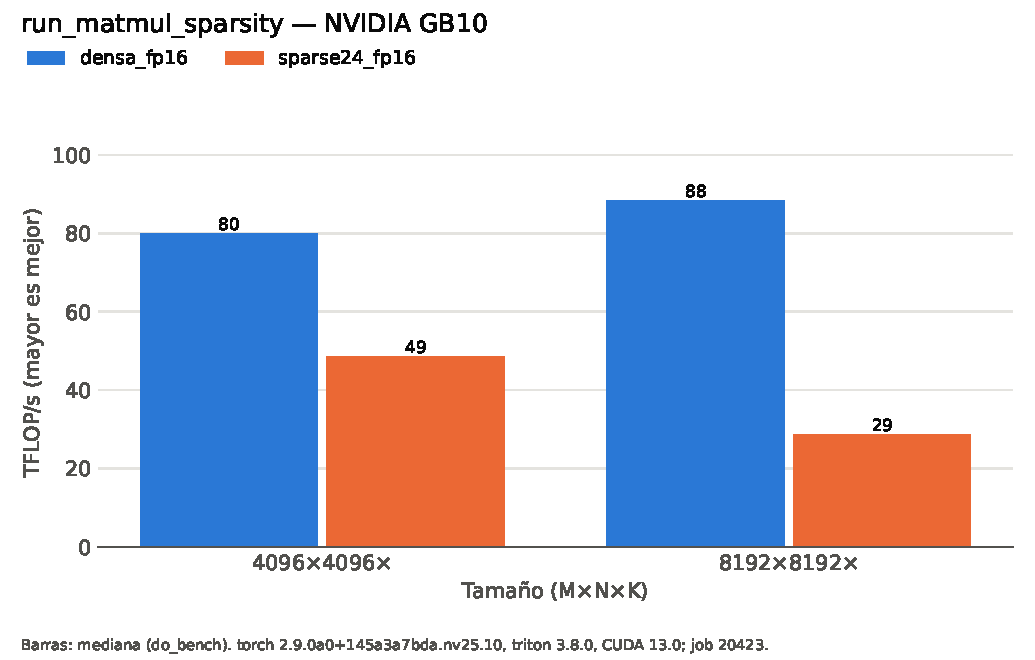
\includegraphics[width=\linewidth]{resultados/hennessy-580/figuras/run_matmul_sparsity.pdf}
  \caption{Matmul en GB10: denso FP16 vs 2:4 sparse FP16 (cuSPARSELt).}
  \label{fig:sparsity}
\end{figure}

\input{resultados/hennessy-580/run_matmul_sparsity.tex}

En $8192^3$: denso 94{,}6 (kernel nativo \texttt{nvjet\_sm121\_\dots\_tmaAB}) vs 2:4 sparse
32{,}3~TFLOP/s (kernel \texttt{sm80\_xmma\_sparse\_gemm}), un 34\,\% del denso. FP8+2:4 da
\texttt{NotImplementedError} (no soportado por la API).

\subsection{Análisis crítico}

\begin{enumerate}
  \item \textbf{El 2:4 no acelera; ralentiza.} El GEMM sparse rinde solo el 34--62\,\% del
  denso, lo contrario del $2\times$ teórico.
  \item \textbf{Falta un kernel sparse nativo de Blackwell.} cuSPARSELt despacha a
  \texttt{sm80\_xmma\_sparse\_gemm} (Ampère), que no explota sm\_121, mientras el denso usa
  un kernel nativo \texttt{nvjet\_sm121\_\dots\_tmaAB} (Blackwell + TMA): el sparse compite
  con hardware de dos generaciones atrás y pierde.
  \item \textbf{FP8 + 2:4 no es accesible} por la API de semi-structured; exigiría bajar a
  cuSPARSELt directamente.
  \item \textbf{El número de catálogo no es reproducible aquí:} los $\sim$838~TFLOPS
  presuponen kernels sparse específicos de la arquitectura (y FP8/FP4) que este \emph{stack}
  todavía no expone para sm\_121.
\end{enumerate}

\subsection{Conclusión}

En GB10 con el \emph{stack} actual, la estructura dispersa 2:4 es una regresión de
rendimiento, no una mejora, por falta de kernel sparse nativo de Blackwell; y la variante
FP8+2:4 no está soportada. La mejor palanca real sigue siendo el FP8 denso
(§~\ref{sec:fp8}): 150~TFLOP/s en Triton y hasta 192 en cuBLASLt, frente a $\sim$92 en FP16.
La sparsity 2:4 queda como línea a revisar cuando el \emph{stack} incorpore kernels sparse
para sm\_121.
.
% Requiere: \usepackage{graphicx,booktabs}. Ajusta rutas si compilas desde otro dir.
% Datos: results/hennessy-580/run_matmul_sparsity/ultimo (job 20402). GB10 (sm_121), torch 2.9.

\section{Estructura dispersa 2:4 en los tensor cores}
\label{sec:sparsity}

La cifra de catálogo de esta clase de GPU ($\sim$838~TFLOPS) es un número \emph{con
sparsity 2:4}: de cada 4 valores, 2 son cero, la matriz se comprime a la mitad más
metadatos, y el circuito sparse del tensor core duplica el throughput saltándose los
ceros. Es, en teoría, la única técnica capaz de superar el techo denso. Se estudia si en
GB10, con el \emph{stack} disponible, ese $2\times$ es alcanzable.

\subsection{Implementación}

Triton no soporta 2:4 en \texttt{tl.dot} (no acepta los metadatos de sparsity), así que se
usa la ruta de PyTorch: se poda A al patrón 2:4 (en cada grupo de 4 a lo largo de K se
conservan los 2 de mayor magnitud), se comprime con
\texttt{torch.sparse.to\_sparse\_semi\_structured} (backend cuSPARSELt) y se mide
\texttt{A\_sp @ B}, comparándolo con el denso \texttt{torch.matmul}. El rendimiento se da
en convención \emph{dense-equivalent} ($2MNK/t$): un $2\times$ real aparecería como
$\sim 2\times$~TFLOP/s.

\subsection{Resultados}

\begin{figure}[htbp]
  \centering
  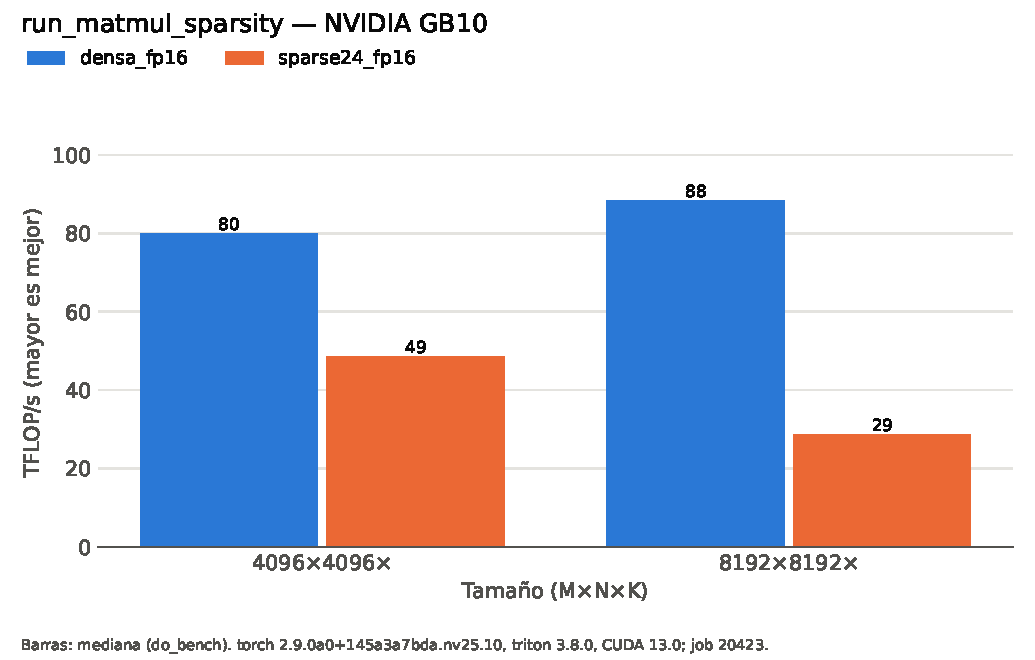
\includegraphics[width=\linewidth]{resultados/hennessy-580/figuras/run_matmul_sparsity.pdf}
  \caption{Matmul en GB10: denso FP16 vs 2:4 sparse FP16 (cuSPARSELt).}
  \label{fig:sparsity}
\end{figure}

% Requiere \usepackage{booktabs}
\begin{table}[htbp]
  \centering\small
  \begin{tabular}{lrrlrrrrrl}
    \toprule
    variante & M & N & K & error\_rel & ms & ms\_p20 & ms\_p80 & tflops & kernel \\
    \midrule
    densa\_fp16 & 4096 & 4096 &  & 0 & 1.7168 & 1.6861 & 1.992 & 80.06 & void cutlass::Kernel2<cutlass\_80\_tensorop\_f16\_s16816gemm\_relu\_f16\_128x256\_32x3\_nn\_align8>(cutlass\_80\_tensorop\_f16\_s16816gemm\_relu\_f16\_128x256\_32x3\_nn\_align8::Params) \\
    sparse24\_fp16 & 4096 & 4096 &  & 4e-05 & 2.8235 & 2.7672 & 2.8826 & 48.68 & sm80\_xmma\_sparse\_gemm\_f16f16\_f16f32\_f32\_tt\_t\_tilesize128x128x64\_stage3\_warpsize2x2x1\_sptensor16x8x32\_execute\_kernel\_5x\_cusparselt \\
    densa\_fp16 & 8192 & 8192 &  & 0 & 12.4518 & 12.331 & 12.7887 & 88.3 & nvjet\_sm121\_hsh\_mma\_128x208x64\_2\_32x104x64\_tmaAB\_bz\_NNNN \\
    sparse24\_fp16 & 8192 & 8192 &  & 6e-05 & 38.463 & 38.0302 & 38.6728 & 28.59 & sm80\_xmma\_sparse\_gemm\_f16f16\_f16f32\_f32\_tt\_t\_tilesize128x128x64\_stage3\_warpsize2x2x1\_sptensor16x8x32\_execute\_kernel\_5x\_cusparselt \\
    \bottomrule
  \end{tabular}
  \caption{run\_matmul\_sparsity: NVIDIA GB10 (sm\_121), torch 2.9.0a0+145a3a7bda.nv25.10, triton 3.8.0, CUDA 13.0; job 20423, 2026-09-30T14:16:29. Mediana de triton.testing.do\_bench.}
  \label{tab:run-matmul-sparsity}
\end{table}


En $8192^3$: denso 94{,}6 (kernel nativo \texttt{nvjet\_sm121\_\dots\_tmaAB}) vs 2:4 sparse
32{,}3~TFLOP/s (kernel \texttt{sm80\_xmma\_sparse\_gemm}), un 34\,\% del denso. FP8+2:4 da
\texttt{NotImplementedError} (no soportado por la API).

\subsection{Análisis crítico}

\begin{enumerate}
  \item \textbf{El 2:4 no acelera; ralentiza.} El GEMM sparse rinde solo el 34--62\,\% del
  denso, lo contrario del $2\times$ teórico.
  \item \textbf{Falta un kernel sparse nativo de Blackwell.} cuSPARSELt despacha a
  \texttt{sm80\_xmma\_sparse\_gemm} (Ampère), que no explota sm\_121, mientras el denso usa
  un kernel nativo \texttt{nvjet\_sm121\_\dots\_tmaAB} (Blackwell + TMA): el sparse compite
  con hardware de dos generaciones atrás y pierde.
  \item \textbf{FP8 + 2:4 no es accesible} por la API de semi-structured; exigiría bajar a
  cuSPARSELt directamente.
  \item \textbf{El número de catálogo no es reproducible aquí:} los $\sim$838~TFLOPS
  presuponen kernels sparse específicos de la arquitectura (y FP8/FP4) que este \emph{stack}
  todavía no expone para sm\_121.
\end{enumerate}

\subsection{Conclusión}

En GB10 con el \emph{stack} actual, la estructura dispersa 2:4 es una regresión de
rendimiento, no una mejora, por falta de kernel sparse nativo de Blackwell; y la variante
FP8+2:4 no está soportada. La mejor palanca real sigue siendo el FP8 denso
(§~\ref{sec:fp8}): 150~TFLOP/s en Triton y hasta 192 en cuBLASLt, frente a $\sim$92 en FP16.
La sparsity 2:4 queda como línea a revisar cuando el \emph{stack} incorpore kernels sparse
para sm\_121.
.
% Requiere: \usepackage{graphicx,booktabs}. Ajusta rutas si compilas desde otro dir.
% Datos: results/hennessy-580/run_matmul_sparsity/ultimo (job 20402). GB10 (sm_121), torch 2.9.

\section{Estructura dispersa 2:4 en los tensor cores}
\label{sec:sparsity}

La cifra de catálogo de esta clase de GPU ($\sim$838~TFLOPS) es un número \emph{con
sparsity 2:4}: de cada 4 valores, 2 son cero, la matriz se comprime a la mitad más
metadatos, y el circuito sparse del tensor core duplica el throughput saltándose los
ceros. Es, en teoría, la única técnica capaz de superar el techo denso. Se estudia si en
GB10, con el \emph{stack} disponible, ese $2\times$ es alcanzable.

\subsection{Implementación}

Triton no soporta 2:4 en \texttt{tl.dot} (no acepta los metadatos de sparsity), así que se
usa la ruta de PyTorch: se poda A al patrón 2:4 (en cada grupo de 4 a lo largo de K se
conservan los 2 de mayor magnitud), se comprime con
\texttt{torch.sparse.to\_sparse\_semi\_structured} (backend cuSPARSELt) y se mide
\texttt{A\_sp @ B}, comparándolo con el denso \texttt{torch.matmul}. El rendimiento se da
en convención \emph{dense-equivalent} ($2MNK/t$): un $2\times$ real aparecería como
$\sim 2\times$~TFLOP/s.

\subsection{Resultados}

\begin{figure}[htbp]
  \centering
  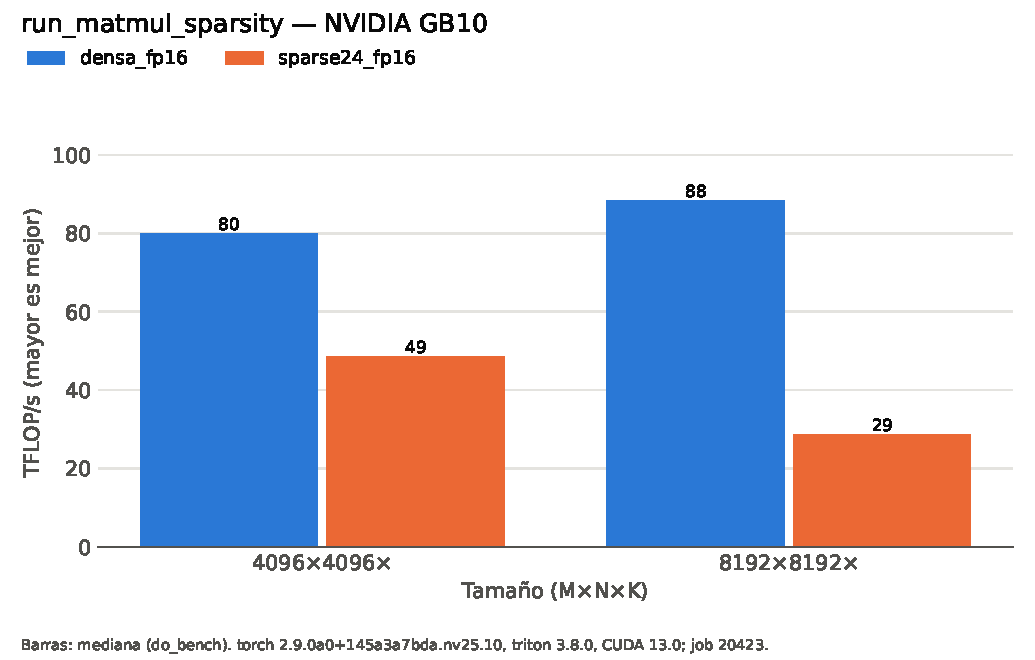
\includegraphics[width=\linewidth]{resultados/hennessy-580/figuras/run_matmul_sparsity.pdf}
  \caption{Matmul en GB10: denso FP16 vs 2:4 sparse FP16 (cuSPARSELt).}
  \label{fig:sparsity}
\end{figure}

% Requiere \usepackage{booktabs}
\begin{table}[htbp]
  \centering\small
  \begin{tabular}{lrrlrrrrrl}
    \toprule
    variante & M & N & K & error\_rel & ms & ms\_p20 & ms\_p80 & tflops & kernel \\
    \midrule
    densa\_fp16 & 4096 & 4096 &  & 0 & 1.7168 & 1.6861 & 1.992 & 80.06 & void cutlass::Kernel2<cutlass\_80\_tensorop\_f16\_s16816gemm\_relu\_f16\_128x256\_32x3\_nn\_align8>(cutlass\_80\_tensorop\_f16\_s16816gemm\_relu\_f16\_128x256\_32x3\_nn\_align8::Params) \\
    sparse24\_fp16 & 4096 & 4096 &  & 4e-05 & 2.8235 & 2.7672 & 2.8826 & 48.68 & sm80\_xmma\_sparse\_gemm\_f16f16\_f16f32\_f32\_tt\_t\_tilesize128x128x64\_stage3\_warpsize2x2x1\_sptensor16x8x32\_execute\_kernel\_5x\_cusparselt \\
    densa\_fp16 & 8192 & 8192 &  & 0 & 12.4518 & 12.331 & 12.7887 & 88.3 & nvjet\_sm121\_hsh\_mma\_128x208x64\_2\_32x104x64\_tmaAB\_bz\_NNNN \\
    sparse24\_fp16 & 8192 & 8192 &  & 6e-05 & 38.463 & 38.0302 & 38.6728 & 28.59 & sm80\_xmma\_sparse\_gemm\_f16f16\_f16f32\_f32\_tt\_t\_tilesize128x128x64\_stage3\_warpsize2x2x1\_sptensor16x8x32\_execute\_kernel\_5x\_cusparselt \\
    \bottomrule
  \end{tabular}
  \caption{run\_matmul\_sparsity: NVIDIA GB10 (sm\_121), torch 2.9.0a0+145a3a7bda.nv25.10, triton 3.8.0, CUDA 13.0; job 20423, 2026-09-30T14:16:29. Mediana de triton.testing.do\_bench.}
  \label{tab:run-matmul-sparsity}
\end{table}


En $8192^3$: denso 94{,}6 (kernel nativo \texttt{nvjet\_sm121\_\dots\_tmaAB}) vs 2:4 sparse
32{,}3~TFLOP/s (kernel \texttt{sm80\_xmma\_sparse\_gemm}), un 34\,\% del denso. FP8+2:4 da
\texttt{NotImplementedError} (no soportado por la API).

\subsection{Análisis crítico}

\begin{enumerate}
  \item \textbf{El 2:4 no acelera; ralentiza.} El GEMM sparse rinde solo el 34--62\,\% del
  denso, lo contrario del $2\times$ teórico.
  \item \textbf{Falta un kernel sparse nativo de Blackwell.} cuSPARSELt despacha a
  \texttt{sm80\_xmma\_sparse\_gemm} (Ampère), que no explota sm\_121, mientras el denso usa
  un kernel nativo \texttt{nvjet\_sm121\_\dots\_tmaAB} (Blackwell + TMA): el sparse compite
  con hardware de dos generaciones atrás y pierde.
  \item \textbf{FP8 + 2:4 no es accesible} por la API de semi-structured; exigiría bajar a
  cuSPARSELt directamente.
  \item \textbf{El número de catálogo no es reproducible aquí:} los $\sim$838~TFLOPS
  presuponen kernels sparse específicos de la arquitectura (y FP8/FP4) que este \emph{stack}
  todavía no expone para sm\_121.
\end{enumerate}

\subsection{Conclusión}

En GB10 con el \emph{stack} actual, la estructura dispersa 2:4 es una regresión de
rendimiento, no una mejora, por falta de kernel sparse nativo de Blackwell; y la variante
FP8+2:4 no está soportada. La mejor palanca real sigue siendo el FP8 denso
(§~\ref{sec:fp8}): 150~TFLOP/s en Triton y hasta 192 en cuBLASLt, frente a $\sim$92 en FP16.
La sparsity 2:4 queda como línea a revisar cuando el \emph{stack} incorpore kernels sparse
para sm\_121.
.
% Requiere: \usepackage{graphicx,booktabs}. Ajusta rutas si compilas desde otro dir.
% Datos: results/hennessy-580/run_matmul_sparsity/ultimo (job 20402). GB10 (sm_121), torch 2.9.

\section{Estructura dispersa 2:4 en los tensor cores}
\label{sec:sparsity}

La cifra de catálogo de esta clase de GPU ($\sim$838~TFLOPS) es un número \emph{con
sparsity 2:4}: de cada 4 valores, 2 son cero, la matriz se comprime a la mitad más
metadatos, y el circuito sparse del tensor core duplica el throughput saltándose los
ceros. Es, en teoría, la única técnica capaz de superar el techo denso. Se estudia si en
GB10, con el \emph{stack} disponible, ese $2\times$ es alcanzable.

\subsection{Implementación}

Triton no soporta 2:4 en \texttt{tl.dot} (no acepta los metadatos de sparsity), así que se
usa la ruta de PyTorch: se poda A al patrón 2:4 (en cada grupo de 4 a lo largo de K se
conservan los 2 de mayor magnitud), se comprime con
\texttt{torch.sparse.to\_sparse\_semi\_structured} (backend cuSPARSELt) y se mide
\texttt{A\_sp @ B}, comparándolo con el denso \texttt{torch.matmul}. El rendimiento se da
en convención \emph{dense-equivalent} ($2MNK/t$): un $2\times$ real aparecería como
$\sim 2\times$~TFLOP/s.

\subsection{Resultados}

\begin{figure}[htbp]
  \centering
  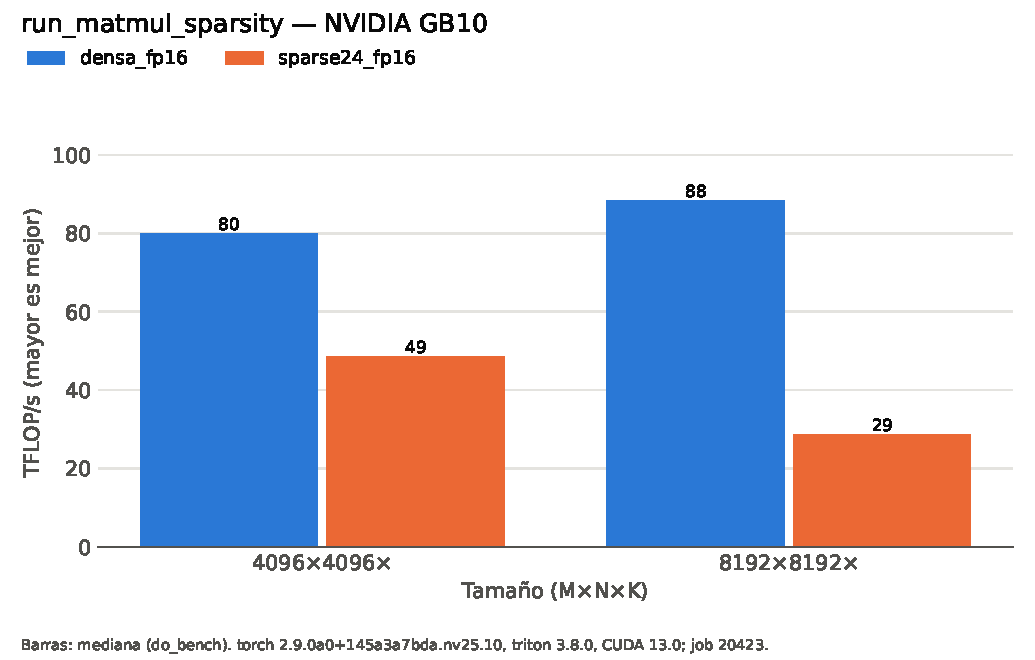
\includegraphics[width=\linewidth]{resultados/hennessy-580/figuras/run_matmul_sparsity.pdf}
  \caption{Matmul en GB10: denso FP16 vs 2:4 sparse FP16 (cuSPARSELt).}
  \label{fig:sparsity}
\end{figure}

% Requiere \usepackage{booktabs}
\begin{table}[htbp]
  \centering\small
  \begin{tabular}{lrrlrrrrrl}
    \toprule
    variante & M & N & K & error\_rel & ms & ms\_p20 & ms\_p80 & tflops & kernel \\
    \midrule
    densa\_fp16 & 4096 & 4096 &  & 0 & 1.7168 & 1.6861 & 1.992 & 80.06 & void cutlass::Kernel2<cutlass\_80\_tensorop\_f16\_s16816gemm\_relu\_f16\_128x256\_32x3\_nn\_align8>(cutlass\_80\_tensorop\_f16\_s16816gemm\_relu\_f16\_128x256\_32x3\_nn\_align8::Params) \\
    sparse24\_fp16 & 4096 & 4096 &  & 4e-05 & 2.8235 & 2.7672 & 2.8826 & 48.68 & sm80\_xmma\_sparse\_gemm\_f16f16\_f16f32\_f32\_tt\_t\_tilesize128x128x64\_stage3\_warpsize2x2x1\_sptensor16x8x32\_execute\_kernel\_5x\_cusparselt \\
    densa\_fp16 & 8192 & 8192 &  & 0 & 12.4518 & 12.331 & 12.7887 & 88.3 & nvjet\_sm121\_hsh\_mma\_128x208x64\_2\_32x104x64\_tmaAB\_bz\_NNNN \\
    sparse24\_fp16 & 8192 & 8192 &  & 6e-05 & 38.463 & 38.0302 & 38.6728 & 28.59 & sm80\_xmma\_sparse\_gemm\_f16f16\_f16f32\_f32\_tt\_t\_tilesize128x128x64\_stage3\_warpsize2x2x1\_sptensor16x8x32\_execute\_kernel\_5x\_cusparselt \\
    \bottomrule
  \end{tabular}
  \caption{run\_matmul\_sparsity: NVIDIA GB10 (sm\_121), torch 2.9.0a0+145a3a7bda.nv25.10, triton 3.8.0, CUDA 13.0; job 20423, 2026-09-30T14:16:29. Mediana de triton.testing.do\_bench.}
  \label{tab:run-matmul-sparsity}
\end{table}


En $8192^3$: denso 94{,}6 (kernel nativo \texttt{nvjet\_sm121\_\dots\_tmaAB}) vs 2:4 sparse
32{,}3~TFLOP/s (kernel \texttt{sm80\_xmma\_sparse\_gemm}), un 34\,\% del denso. FP8+2:4 da
\texttt{NotImplementedError} (no soportado por la API).

\subsection{Análisis crítico}

\begin{enumerate}
  \item \textbf{El 2:4 no acelera; ralentiza.} El GEMM sparse rinde solo el 34--62\,\% del
  denso, lo contrario del $2\times$ teórico.
  \item \textbf{Falta un kernel sparse nativo de Blackwell.} cuSPARSELt despacha a
  \texttt{sm80\_xmma\_sparse\_gemm} (Ampère), que no explota sm\_121, mientras el denso usa
  un kernel nativo \texttt{nvjet\_sm121\_\dots\_tmaAB} (Blackwell + TMA): el sparse compite
  con hardware de dos generaciones atrás y pierde.
  \item \textbf{FP8 + 2:4 no es accesible} por la API de semi-structured; exigiría bajar a
  cuSPARSELt directamente.
  \item \textbf{El número de catálogo no es reproducible aquí:} los $\sim$838~TFLOPS
  presuponen kernels sparse específicos de la arquitectura (y FP8/FP4) que este \emph{stack}
  todavía no expone para sm\_121.
\end{enumerate}

\subsection{Conclusión}

En GB10 con el \emph{stack} actual, la estructura dispersa 2:4 es una regresión de
rendimiento, no una mejora, por falta de kernel sparse nativo de Blackwell; y la variante
FP8+2:4 no está soportada. La mejor palanca real sigue siendo el FP8 denso
(§~\ref{sec:fp8}): 150~TFLOP/s en Triton y hasta 192 en cuBLASLt, frente a $\sim$92 en FP16.
La sparsity 2:4 queda como línea a revisar cuando el \emph{stack} incorpore kernels sparse
para sm\_121.
